\documentclass{article}
\usepackage{tikz}
\usetikzlibrary{fit,positioning}
\usetikzlibrary{shapes,arrows}

\begin{document}

\begin{tikzpicture}
\begin{scope}[shift={(1,1)},local bounding box=A]
\draw (0,0) rectangle (11.3,1.5);
\draw (0.2,0.2) rectangle (3.2,1);
\draw (3.7,0.2) rectangle (6.7,1);
\draw (7.2,0.2) rectangle (10.2,1);
\node[scale=0.8] at (1.65,0.5) {$S_{x_{1}}$};
\node[scale=0.8] at (5.5,0.5) {$S_{x_{2}}$};
\node[scale=0.8] at (8.5,0.5) {$S_{x_{3}}$};
\node[scale=0.8] at (10.65,0.5) {$S_{x}$};
\end{scope}
\draw[->] (0,0) -- (A.west);
\end{tikzpicture}









\begin{center}
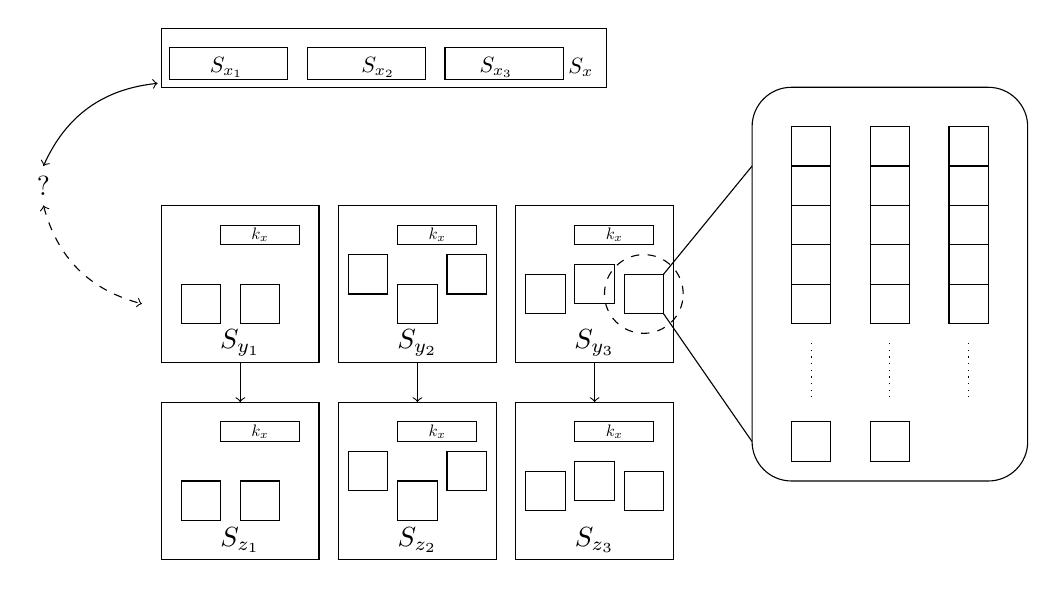
\begin{tikzpicture}[scale=0.5]

\draw (0,0) -- (0,1.5) -- (11.3,1.5) -- (11.3,0) -- cycle;
\draw (0.2,0.2) -- (0.2,1) -- (3.2,1) -- (3.2,0.2) -- cycle;
\draw (3.7,0.2) -- (3.7,1) -- (6.7,1) -- (6.7,0.2) -- cycle;
\draw (7.2,0.2) -- (7.2,1) -- (10.2,1) -- (10.2,0.2) -- cycle;

\node[scale=0.8] at (1.65,0.5) {$S_{x_{1}}$};
\node[scale=0.8] at (5.5,0.5) {$S_{x_{2}}$};
\node[scale=0.8] at (8.5,0.5) {$S_{x_{3}}$};
\node[scale=0.8] at (10.65,0.5) {$S_{x}$};

\draw [<->] (-0.1,0.1) to [bend right] (-3,-2);
\node at (-3,-2.5) {?};
\draw [<->, dashed] (-3,-3) to [bend right] (-0.5,-5.5);

\draw (0,-7) -- (0,-3) -- (4,-3) -- (4,-7) -- cycle;
\draw (1.5,-3.5) -- (3.5,-3.5) -- (3.5,-4) -- (1.5,-4) -- cycle;
\draw (0.5,-6) -- (0.5,-5) -- (1.5,-5) -- (1.5,-6) -- cycle;
\draw (2,-6) -- (2,-5) -- (3,-5) -- (3,-6) -- cycle;
\node [scale=0.6] at (2.5,-3.75) {$k_{x}$};
\node at (2,-6.5) {$S_{y_{1}}$};

\draw (4.5,-7) -- (4.5,-3) -- (8.5,-3) -- (8.5,-7) -- cycle;
\draw (6,-3.5) -- (8,-3.5) -- (8,-4) -- (6,-4) -- cycle;
\draw (6,-6) -- (6,-5) -- (7,-5) -- (7,-6) -- cycle;
\draw (4.75,-5.25) -- (4.75,-4.25) -- (5.75,-4.25) -- (5.75,-5.25) -- cycle;
\draw (7.25,-5.25) -- (7.25,-4.25) -- (8.25,-4.25) -- (8.25,-5.25) -- cycle;
\node [scale=0.6] at (7,-3.75) {$k_{x}$};
\node at (6.5,-6.5) {$S_{y_{2}}$};

\draw (9,-7) -- (9,-3) -- (13,-3) -- (13,-7) -- cycle;
\draw (10.5,-3.5) -- (12.5,-3.5) -- (12.5,-4) -- (10.5,-4) -- cycle;
\draw (10.5,-5.5) -- (10.5,-4.5) -- (11.5,-4.5) -- (11.5,-5.5) -- cycle;
\draw (9.25,-5.75) -- (9.25,-4.75) -- (10.25,-4.75) -- (10.25,-5.75) -- cycle;
\draw (11.75,-5.75) -- (11.75,-4.75) -- (12.75,-4.75) -- (12.75,-5.75) -- cycle;
\node [scale=0.6] at (11.5,-3.75) {$k_{x}$};
\node at (11,-6.5) {$S_{y_{3}}$};

\draw (0,-12) -- (0,-8) -- (4,-8) -- (4,-12) -- cycle;
\draw (1.5,-8.5) -- (3.5,-8.5) -- (3.5,-9) -- (1.5,-9) -- cycle;
\draw (0.5,-11) -- (0.5,-10) -- (1.5,-10) -- (1.5,-11) -- cycle;
\draw (2,-11) -- (2,-10) -- (3,-10) -- (3,-11) -- cycle;
\node [scale=0.6] at (2.5,-8.75) {$k_{x}$};
\node at (2,-11.5) {$S_{z_{1}}$};

\draw (4.5,-12) -- (4.5,-8) -- (8.5,-8) -- (8.5,-12) -- cycle;
\draw (6,-8.5) -- (8,-8.5) -- (8,-9) -- (6,-9) -- cycle;
\draw (6,-11) -- (6,-10) -- (7,-10) -- (7,-11) -- cycle;
\draw (4.75,-10.25) -- (4.75,-9.25) -- (5.75,-9.25) -- (5.75,-10.25) -- cycle;
\draw (7.25,-10.25) -- (7.25,-9.25) -- (8.25,-9.25) -- (8.25,-10.25) -- cycle;
\node [scale=0.6] at (7,-8.75) {$k_{x}$};
\node at (6.5,-11.5) {$S_{z_{2}}$};

\draw (9,-12) -- (9,-8) -- (13,-8) -- (13,-12) -- cycle;
\draw (10.5,-8.5) -- (12.5,-8.5) -- (12.5,-9) -- (10.5,-9) -- cycle;
\draw (10.5,-10.5) -- (10.5,-9.5) -- (11.5,-9.5) -- (11.5,-10.5) -- cycle;
\draw (9.25,-10.75) -- (9.25,-9.75) -- (10.25,-9.75) -- (10.25,-10.75) -- cycle;
\draw (11.75,-10.75) -- (11.75,-9.75) -- (12.75,-9.75) -- (12.75,-10.75) -- cycle;
\node [scale=0.6] at (11.5,-8.75) {$k_{x}$};
\node at (11,-11.5) {$S_{z_{3}}$};

\draw [->] (2,-7) -- (2,-8);
\draw [->] (6.5,-7) -- (6.5,-8);
\draw [->] (11,-7) -- (11,-8);

\draw [dashed] (12.25,-5.25) circle (1cm);

\draw (12.75,-4.75) -- (15,-2);
\draw (12.75,-5.75) -- (15,-9);

\draw [rounded corners=.5cm] (15,-10) -- (15,0) -- (22,0) -- (22,-10) -- cycle;
\draw (16,-1) -- (17,-1) -- (17,-6) -- (16,-6) -- cycle;
\draw (16,-2) -- (17,-2);
\draw (16,-3) -- (17,-3);
\draw (16,-4) -- (17,-4);
\draw (16,-5) -- (17,-5);
\draw (18,-1) -- (19,-1) -- (19,-6) -- (18,-6) -- cycle;
\draw (18,-2) -- (19,-2);
\draw (18,-3) -- (19,-3);
\draw (18,-4) -- (19,-4);
\draw (18,-5) -- (19,-5);
\draw (20,-1) -- (21,-1) -- (21,-6) -- (20,-6) -- cycle;
\draw (20,-2) -- (21,-2);
\draw (20,-3) -- (21,-3);
\draw (20,-4) -- (21,-4);
\draw (20,-5) -- (21,-5);

\draw [dotted] (16.5,-6.5) -- (16.5,-8);
\draw [dotted] (18.5,-6.5) -- (18.5,-8);
\draw [dotted] (20.5,-6.5) -- (20.5,-8);

\draw (16,-8.5) -- (17,-8.5) -- (17,-9.5) -- (16,-9.5) -- cycle;
\draw (18,-8.5) -- (19,-8.5) -- (19,-9.5) -- (18,-9.5) -- cycle;
\end{tikzpicture}
\end{center}






% Define block styles
\tikzstyle{decision} = [diamond, draw, fill=blue!20, 
    text width=4.5em, text badly centered, node distance=3cm, inner sep=0pt]
\tikzstyle{block} = [rectangle, draw, fill=blue!20, 
    text width=5em, text centered, rounded corners, minimum height=4em]
\tikzstyle{line} = [draw, -latex']
\tikzstyle{cloud} = [draw, ellipse,fill=red!20, node distance=3cm,
    minimum height=2em]

\begin{tikzpicture}[node distance = 2cm, auto]
    % Place nodes
    \node [block] (init) {initialize model};
    \node [cloud, left of=init] (expert) {expert};
    \node [cloud, right of=init] (system) {system};
    \node [block, below of=init] (identify) {identify candidate models};
    \node [block, below of=identify] (evaluate) {evaluate candidate models};
    \node [block, left of=evaluate, node distance=3cm] (update) {update model};
    \node [decision, below of=evaluate] (decide) {is best candidate better?};
    \node [block, below of=decide, node distance=3cm] (stop) {stop};
    % Draw edges
    \path [line] (init) -- (identify);
    \path [line] (identify) -- (evaluate);
    \path [line] (evaluate) -- (decide);
    \path [line] (decide) -| node [near start] {yes} (update);
    \path [line] (update) |- (identify);
    \path [line] (decide) -- node {no}(stop);
    \path [line,dashed] (expert) -- (init);
    \path [line,dashed] (system) -- (init);
    \path [line,dashed] (system) |- (evaluate);
\end{tikzpicture}










% Define block styles
\tikzstyle{decision} = [diamond, draw, fill=white!20, 
    text width=4.5em, text badly centered, node distance=3cm, inner sep=0pt]
\tikzstyle{block} = [rectangle, draw, fill=white!20, 
    text width=5em, text centered, rounded corners, minimum height=4em]
\tikzstyle{line} = [draw, -latex']
\tikzstyle{cloud} = [draw, ellipse,fill=white!20, node distance=3cm,
    minimum height=2em]

\begin{tikzpicture}[node distance = 2cm, auto]
    % Place nodes
    \node [block] (init) {initialize model};
    \node [cloud, left of=init] (expert) {expert};
    \node [cloud, right of=init] (system) {system};
    \node [block, below of=init] (identify) {identify candidate models};
    \node [block, below of=identify] (evaluate) {evaluate candidate models};
    \node [block, left of=evaluate, node distance=3cm] (update) {update model};
    \node [decision, below of=evaluate] (decide) {is best candidate better?};
    \node [block, below of=decide, node distance=3cm] (stop) {stop};
    % Draw edges
    \path [line] (init) -- (identify);
    \path [line] (identify) -- (evaluate);
    \path [line] (evaluate) -- (decide);
    \path [line] (decide) -| node [near start] {yes} (update);
    \path [line] (update) |- (identify);
    \path [line] (decide) -- node {no}(stop);
    \path [line,dashed] (expert) -- (init);
    \path [line,dashed] (system) -- (init);
    \path [line,dashed] (system) |- (evaluate);
\end{tikzpicture}














\end{document}